\noindent This chapter is intended as a brief introduction to the laser spectroscopy experiment present at TRIUMF, with special emphasis on the parts relevant to this work. A more complete description of the experiment can be found in \cite{CFBS}.

As stated in the previous chapter, collinear laser spectroscopy operates by bringing a particle beam into resonance, through Doppler tuning, with a co-propagating (or counter-propagating, as is the case at TRIUMF) laser, which excites transitions in the electronic structure of the particles. The photons that are produced as a result of the de-excitation are then measured by light collection instruments. Located in the ISAC I (Isotope Separator and ACcelerator) experimental hall at TRIUMF, as shown in Fig. \ref{loc}, the Laser Spectroscopy experiment at TRIUMF, more specifically known as the Collinear Fast-Beam laser Spectroscopy (CFBS) experiment, is shown in Fig. \ref{exp}. 


\begin{figure}[h]
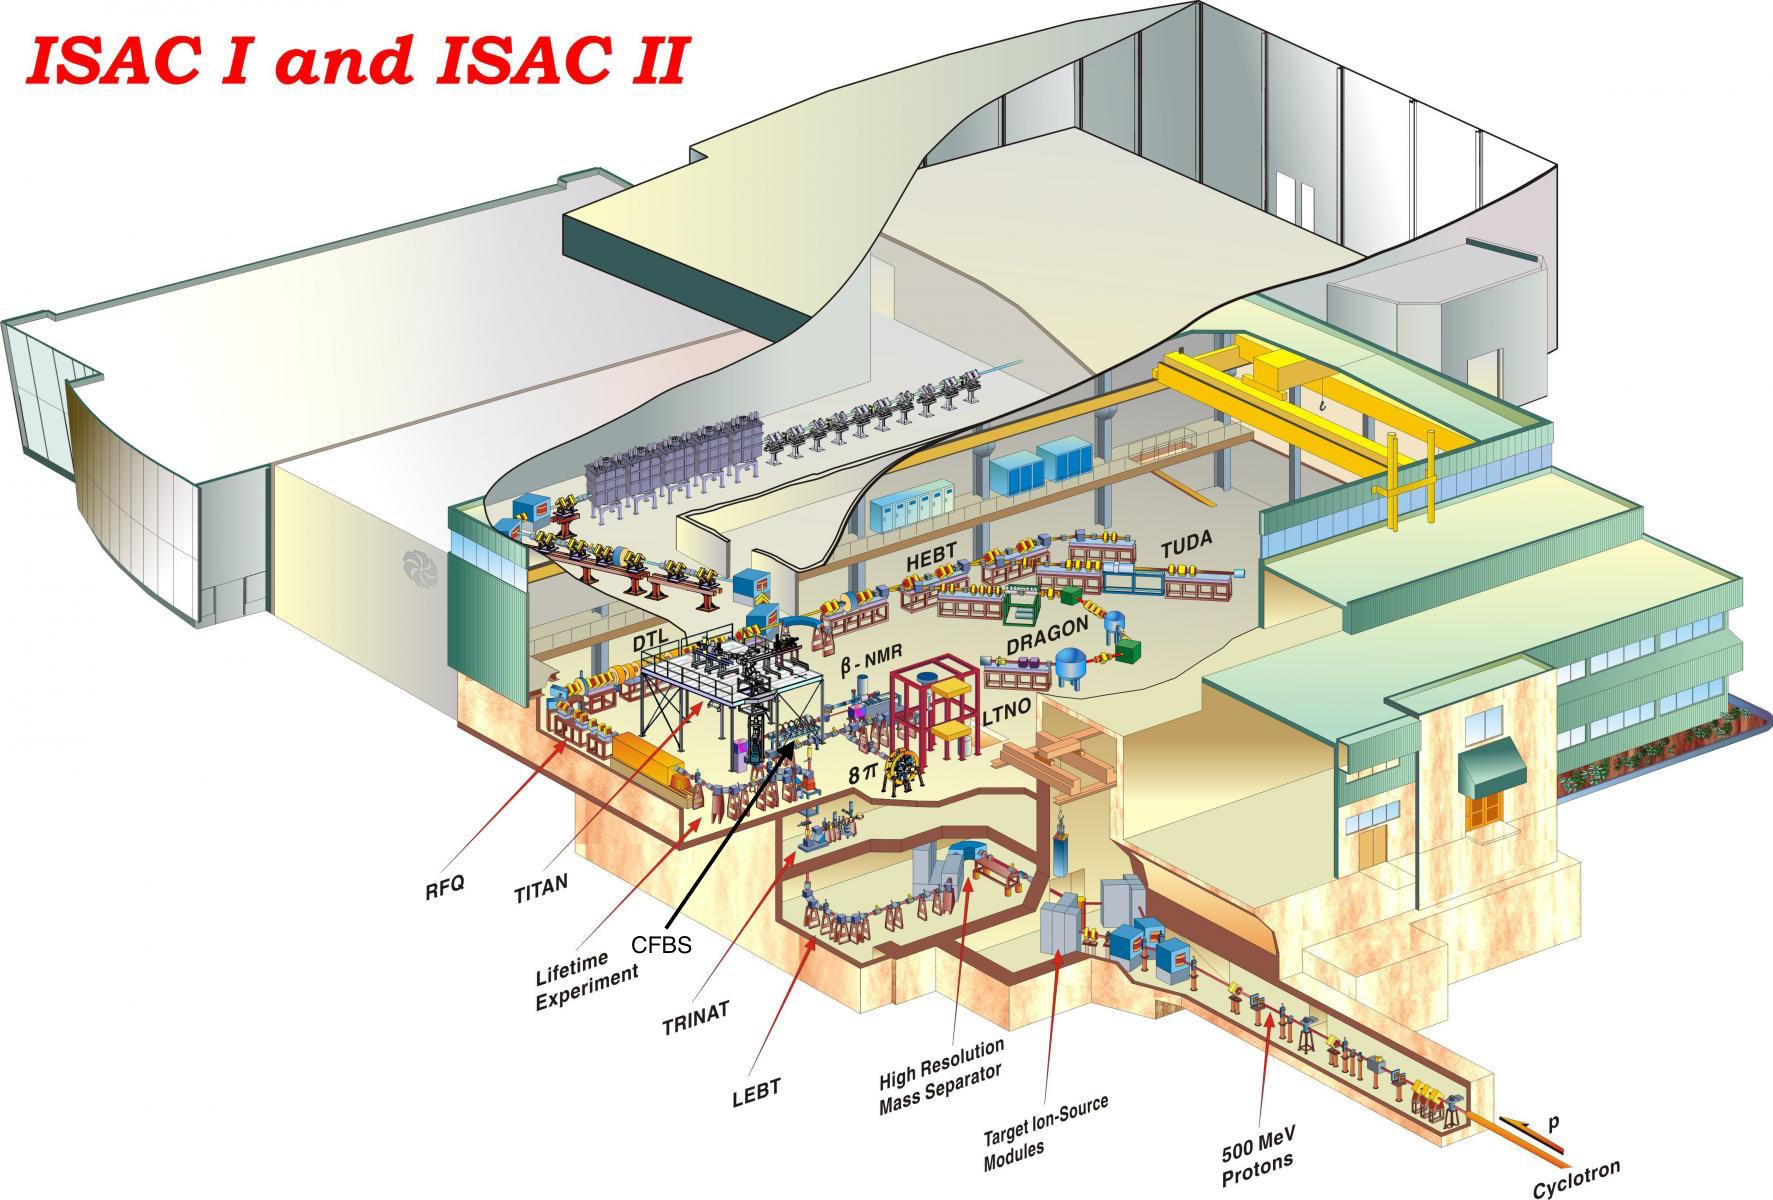
\includegraphics[width=\textwidth]{Laser_spec_triumf/ISAC.png}
\caption[The location of the CFBS experiment]{\small The location of the CFBS experiment within the ISAC I experimental hall, as well as the locations of the beamline and other experiments present at TRIUMF\cite{CFBS}.}
\label{loc}
\end{figure}

\begin{figure}[h]
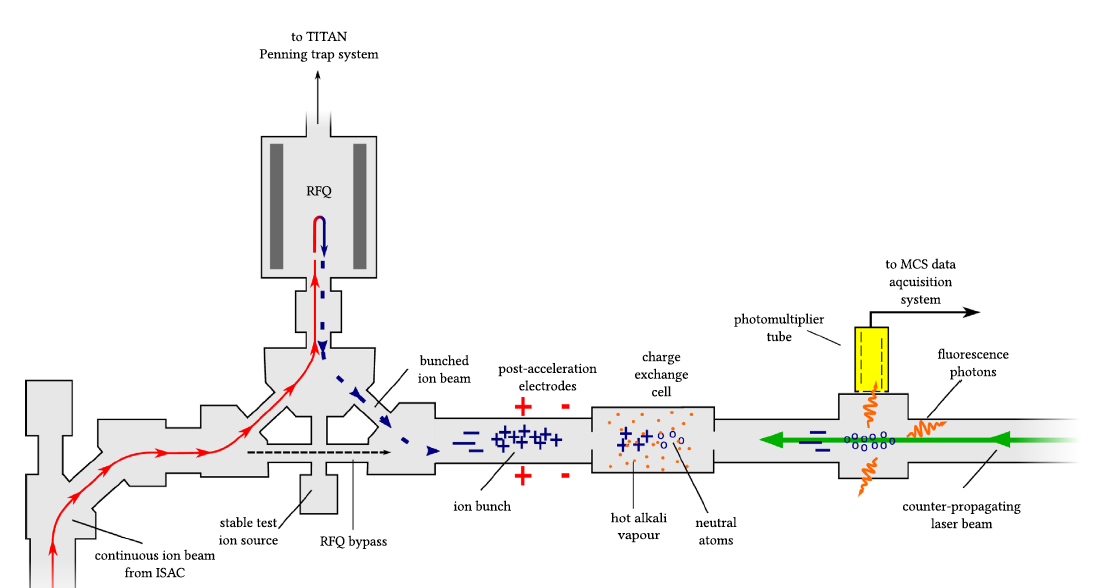
\includegraphics[width=\textwidth]{Laser_spec_triumf/experiment.png}
\caption[Schematic of the CFBS experiment at TRIUMF]{\small Schematic of the CFBS experiment at TRIUMF. Radioactive ions produced in the target area are accelerated towards the experiment\cite{CFBS}.}
\label{exp}
\end{figure}

At TRIUMF, radioactive atoms are produced by 500 MeV protons impinging on a heavy target, inducing spallation. The products of the spallation then diffuse out of the target material, effuse from the target to the ion source, where they are ionized, accelerated and mass separated using a mass separator with resolution $m/\Delta m \approx 2000$, where $m$ is the mass of the atom\cite{CFBS}. After the required atoms have been selected, they are then directed to the CFBS experiment, detailed below. In general, the CFBS group studies very exotic ions, i.e. ions that have low production rates.

\section{Radio Frequency Quadrupole (RFQ) Trap}

The ions enter the CFBS experiment as a continuous beam, where they first encounter a radio frequency quadrupole (RFQ) Paul Trap\cite{CFBS}. Here, the atoms can enter the RFQ trap and are collected for a pre-determined collection time, after which they are released in bunches. Bunching the atoms helps to significantly reduce background counts. Briefly, the light collection system is triggered on the release of the ion bunches, reducing the available time for background photons to be counted. As the light collection system is only sensitive to photons for the time window during which the ion bunch passes through the interaction region, background counts are also only collected for this time. Alternatively, photons are collected continuously, whether or not there are ions in the interaction region, allowing the signal to noise ratio to diminish over time. Ideally, the two methods produce the same signal, but with the latter having a significantly higher background. In general, the background is formed by dark counts from the photo-multiplier and actual photons scattered around the vacuum system. When continuously collected, the background is the rate of these events multiplied by the collection time. When the beam is pulsed, the background is the rate of the background events times the pulse length times the number of pulses per second. A typical pulse length is roughly 10$\mu s$ at about 100 pulses per second\cite{CFBS}.

\section{Charge Exchange Cell (CEC)}
If the aim is to investigate transitions in a neutral atom, then the ions must regain their lost electron. This is the role of the charge exchange cell (CEC), shown in detail in Fig. \ref{CEC}. Using an alkali-metal vapour that is circulated perpendicularly to the direction of the beam, the CEC provides a source of electrons for the oncoming ions to capture. This introduces an issue, however. As the alkali-metal vapour can not be entirely contained to the CEC, any light collection instruments, such as a photo-multiplier tube,  must be located further down the beamline. This is done to avoid the growth of an alkali-metal coating on the light-collection surfaces which would significantly hamper the collection of resonant photons as the experiment progresses. This decision provides the \emph{raison d'être} for this work, as it introduces the opportunity for optical pumping, discussed in detail in Chapter \ref{Op_pump}. Since the ions are neutralized in the CEC, they can no longer be accelerated through the use of an electrostatic potential. As such, they must be brought into resonance before they enter the interaction region. This is done using a set of electrodes present in front of the CEC, shown in Fig. \ref{exp}, as well as floating the CEC.

In the case of transitions present in the ion, then the CEC is unneeded, and the final acceleration is done using a mesh present within the LCR, detailed in the next section. The location of the mesh is chosen such that the ions are in resonance just as they pass the light collection system, removing the possibility that optical pumping could significantly affect the results of the experiment. 



\begin{figure}[h]
\begin{center}
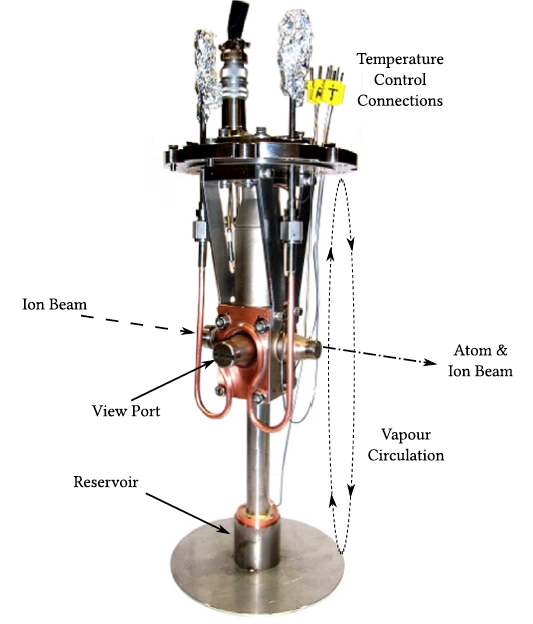
\includegraphics[scale=0.55]{Laser_spec_triumf/CEC.png}
\end{center}
\caption[The charge exchange cell.]{\small The charge exchange cell allows oncoming ions to be neutralized through collision with a perpendicularly flowing alkali-metal vapour\citep{CFBS}.}
\label{CEC}
\end{figure}



\section{Light Collection Region (LCR)}

Located roughly 40 cm down the beamline from the CEC, the light collection region (LCR) (Fig. \ref{LCR}) houses the equipment necessary for detecting the photons emitted when a beam of ions/atoms is in resonance with a counter propagating laser. A concave mirror located opposite the photo-multiplier tube (PMT) allows all photons within the 5\% solid angle of the detection system to be collected by a series of light collection optics, placed in front of the PMT, designed to optimize photon detection efficiency at a particular wavelength\cite{CFBS}. Using knowledge of the laser frequency, the beam energy and photon counts, the energies of the hyperfine transitions can be determined. 
\begin{figure}[t!]
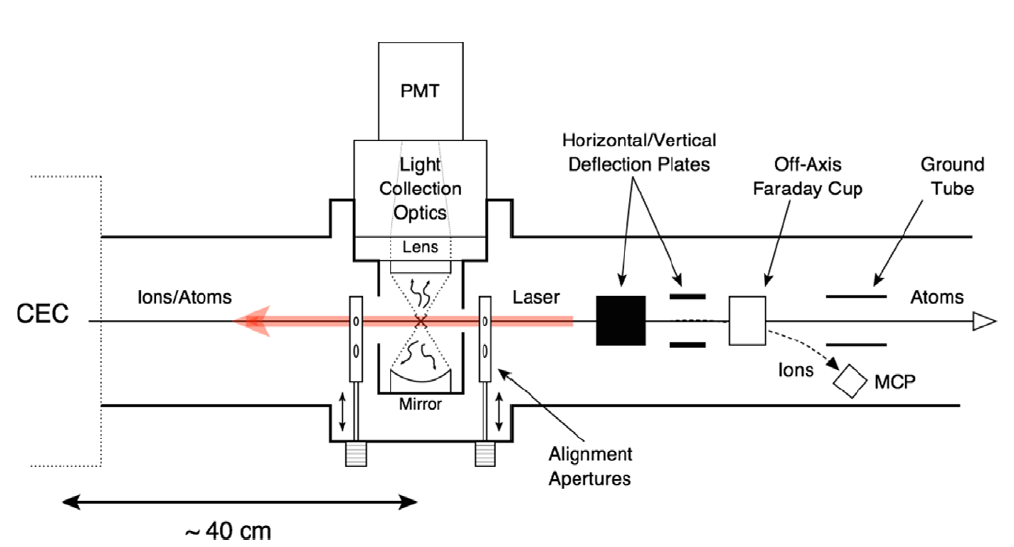
\includegraphics[scale=0.35]{Laser_spec_triumf/LCR.png}
\caption[Schematic of the light collection region.]{\small Schematic of the light collection region. Photons emitted through atom/laser interactions are directed towards a photo-multiplier tube using a combination of mirrors and lenses\citep{CFBS}.}
\label{LCR}
\end{figure}
